\section{Calibration}

This section describes the procedures used to obtain preliminary energy and timing calibarations of the FEC in preparation for the CLAS12 engineering and initial experimental physics runs in 2017-2018.  Although calibration algorithms were already honed from experience with CLAS, some additional complexity was introduced by the addition of PCAL and the requirements of the FPGA-based physics triggers: 

$\bullet$ Differences in the U,V,W readout geometry of PCAL imposed the need to incorporate light attenuation corrections in the trigger firmware to ensure efficiency and spatial uniformity in the cluster energy reconstruction.

$\bullet$ Trigger efficiency studies and overall physics requirements required well-defined cluster energy thresholds for both electron and MIP triggers in each calorimeter layer (PCAL,ECIN,ECOU).

$\bullet$ Introduction of WLS fibers in the PCAL readout required more accurate time-walk corrections to compensate for the slower scintillator risetimes in the PMT pulse.

\subsection{Energy calibration}
The longitudinal and transverse segmentation of the FEC modules together with the requirement for pattern recognition in the hodoscope design means that cluster reconstruction from the full detector involves a minimum of 9 and up to 25 PMTs.  The total detected energy $E_{det}$ results from the summation:
\begin{equation}
 E_{det} = \sum_{s}^{3} \sum_{v}^{3} \sum_{n}^{N} E_{n}^{sv}\label{eq:E1}
\end{equation}
\begin{equation}
 E_{n}^{sv} = k(A_{sig}-A_{ped})/(a+c e^{-xb})   \label{eq:E2}
\end{equation}
\begin{equation}
 E_{tot} = E_{det}/f_{s}                 \label{eq:E3}
\end{equation}
where $E_{n}^{sv}$ is the measured energy in the $\it{nth}$ PMT contributing to the peak 
in view $\it{v}$ and stack $\it{s}$, and $\it{k}$ is a conversion from fADC units to MeV.  The summation occurs over the N PMTs in each peak, over the 3 U,V,W views for each stack, and over the PCAL, ECIN and ECOU stacks.  The measured quantities are $\it{A_{sig}}$, the integrated digitized PMT pulse from the fADC and $\it{A_{ped}}$, the fADC pedestal.  The unknown quantities are the constants $a,b,c$ for the parameterization of the light attenuation as a function of the distance $\it{x}$ from the cluster to the readout end of scintillator strip. For EM showers, the detected energy must be corrected by the sampling fraction $f_{s}$, to obtain the total deposited energy $E_{tot}$.  

Since the energy of an electron incident on the FEC is known from forward tracking, energy calibration of the FEC is in principle possible by adjusting the $a,b,c$ parameters and the sampling fraction $f_{s}$ until the reconstructed energy matches the known energy.  However compared to conventional readout geometries, the relationship in the FEC between the total deposited energy $E_{tot}$ and the partial energies $E_{n}^{sv}$ is non-trivial for EM showers.  A global optimization would require fitting hundreds of parameters per sector and might be very slow to converge.

A simpler approach used successfully in CLAS with the EC is to proceed iteratively, using minimum ionizing particles (MIP) such as cosmic muons to simplify the energy deposition profile and allow an independent determination of the $a,b,c$ parameters for each PMT, then adjust the PMT HV to produce a uniform overall response.  Later, beam data taken with electrons and pions is used to estimate $\it{f_s}$ and to cross-check the MIP calibration.  With the addition of PCAL to CLAS12 and the introduction of cluster reconstruction in the trigger, pre-calibration with cosmics is critical for evaluating the trigger performance of the FEC.

Cosmic runs are performed using a special FPGA trigger that accepts only events where a single pixel has been activated. A pixel is the simplest possible cluster, and is the smallest unit of x-y position resolution in the FEC calorimeters, defined by the overlap of 3 scintillator stacks, one from each of the U,V and W views.  Requiring the muon to pass through a single pixel places the most restrictive cut possible on the particle track path length, thereby minimizing the spread in the MIP energy deposition.   
\begin{figure}[hbt]
\centering
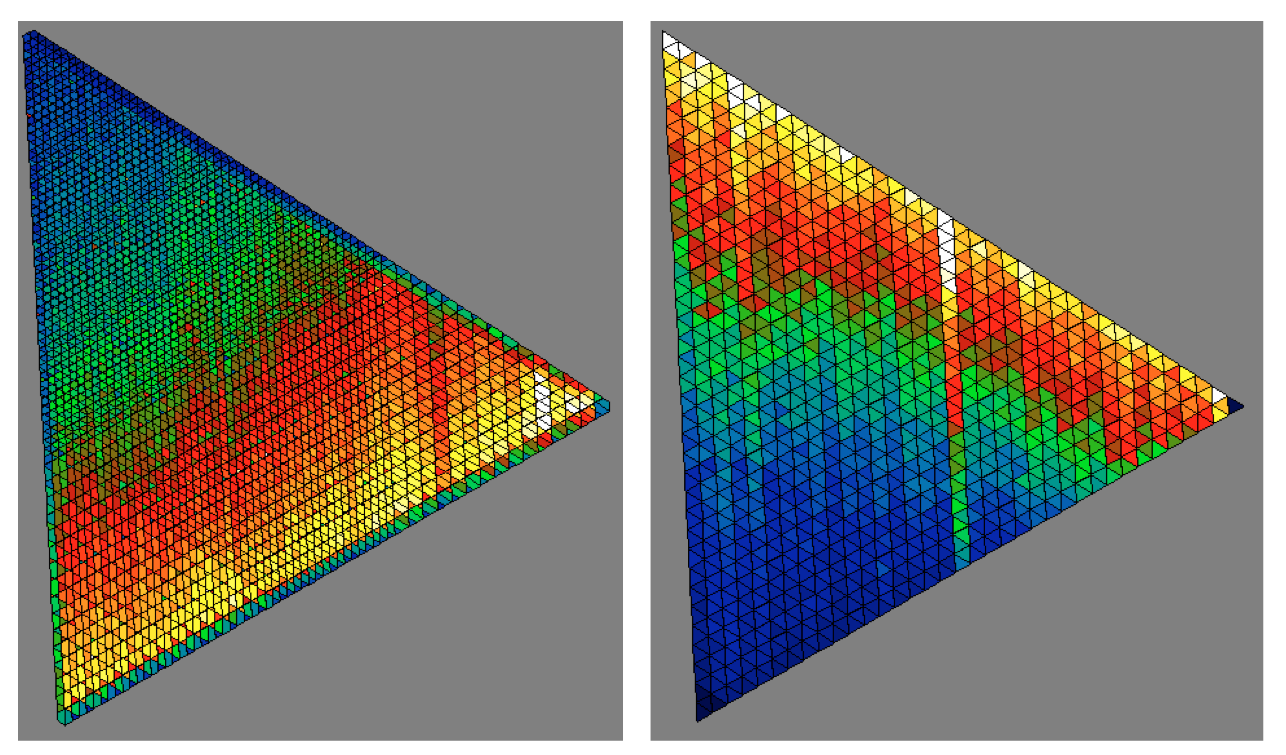
\includegraphics[width=1.0\columnwidth,keepaspectratio]{img/S9_1.png}
\caption[]{Pixel map of mean energy loss from MIP muons measured in Sector 5 W PMTs in PCAL (left) and ECIN (right). Note in PCAL both V and W PMTs are readout from the base of the triangle, while ECIN W PMTs are readout along the right side.  Color gradient from yellow to blue shows the light attenuation as a function of increasing distance from the readout end of each scintillator. }
\label{fig:S9_1}
\end{figure}

A pixel map of the FEC response to cosmic pixel triggers is shown in Fig.~\ref{fig:S9_1} for W view strips in PCAL (left) and ECIN (right). The color gradient in both plots clearly shows the attenuation of light as a function of readout distance from the pixel, as well as overall variations in PMT gain near the readout end, such as the substantially brighter strip in ECIN W19.  Also evident is the finer granularity of pixels in PCAL compared to ECIN.  Note also that unlike the ECIN and ECOU calorimeters, which have a constant pixel size, the PCAL pixels have a variable size and shape due to the mixture of single and double readout strip widths and the different number of readout strips in U compared to V and W. 
\begin{figure}[hbt]
\centering
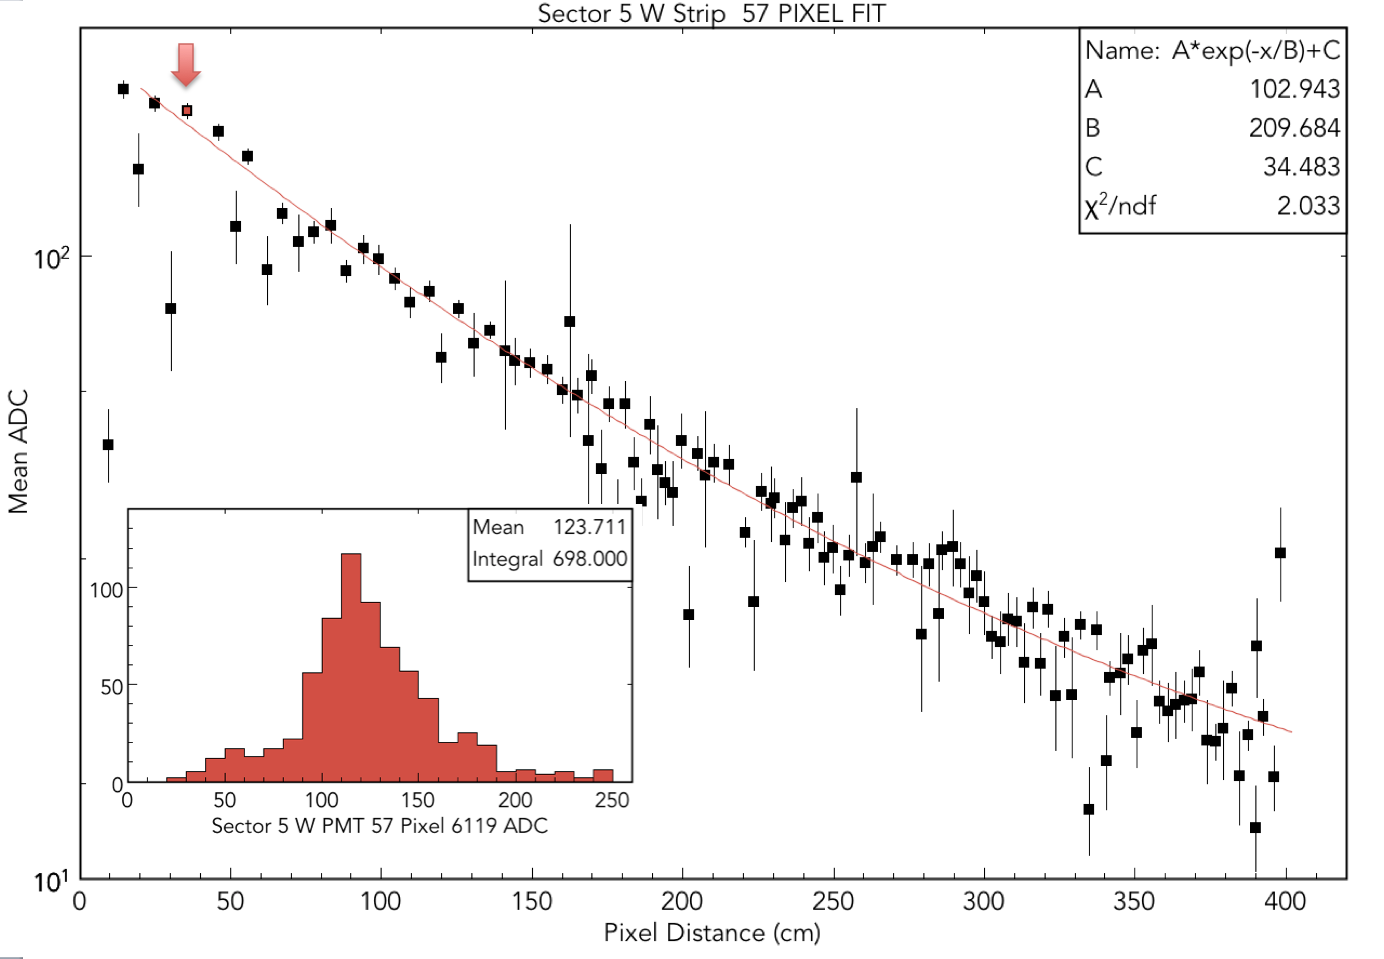
\includegraphics[width=1.0\columnwidth,keepaspectratio]{img/S9_2.png}
\caption[]{Typical fits to muon MIP mean energy loss in PCAL pixels as a function of pixel distance from readout end of strip. Inset shows energy loss distribution in fADC units for the pixel highlighted by the arrow at top.}
\label{fig:S9_2}
\end{figure}

A typical attenuation response plot for a single PCAL PMT (W57) is shown in Fig.~\ref{fig:S9_2} from a cosmic run using a PCAL pixel trigger.  The inset shows the energy loss distribution from a single pixel near the readout end of the scintillator stack and the mean of this distribution for each pixel are the points plotted in the main figure.  The fit shown is used to obtain the $\it{a,b,c}$ calibration constants discussed above, and the goal of this calibration was to normalize all PMT gains with HV adjustments until the quantity $\it{a+c}$ was equal to 150.  

\subsection{Timing calibration}




